\documentclass[10pt, compress]{beamer}

\usetheme{m}

\usepackage{booktabs}
\usepackage[scale=2]{ccicons}
\usepackage{minted}
\usemintedstyle{trac}

\title{Association of large scale\protect\\spatial autocorrelation of aquatic insect trait distribution with climate}
\subtitle{}
\date{\today}
\author{Avit Kumar Bhowmik}
\institute{Institute for Environmental Sciences, University of Koblenz-Landau \protect\\ \protect\\}
 $\vcenter{\hbox{
\includegraphics[width=0.25\textwidth]{images/logo.png}}}$
 \hspace{10pt}
$\vcenter{\hbox{
\includegraphics[width=0.7\textwidth]{images/logo_conference.png}}}$

\begin{document}

\maketitle

\begin{frame}%[fragile]
  \frametitle{Climate is the predominent driver of freshwater assemblages \protect\\ on large scales \small{(Conti et al. 2013, Poff et al. 2010)}}

  %The \emph{mtheme} is a Beamer theme with minimal visual noise inspired by the
  %\href{https://github.com/hsrmbeamertheme/hsrmbeamertheme}{\textsc{hsrm} Beamer
  %Theme} by Benjamin Weiss.

  %Enable the theme by loading

  %\begin{minted}[fontsize=\small]{latex}
    %\documentclass{beamer}
    %\usetheme{m}
  %\end{minted}

  %Note, that you have to have Mozilla's \emph{Fira Sans} font and XeTeX
  %installed to enjoy this wonderful typography.
\centering
  $\vcenter{\hbox{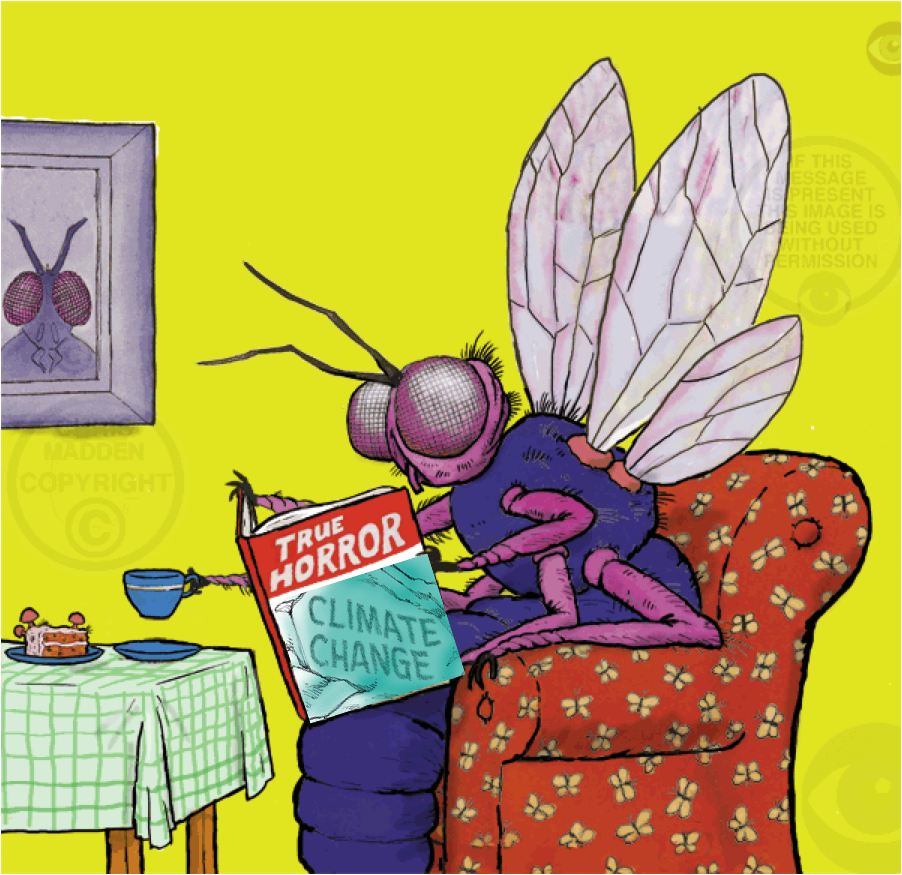
\includegraphics[width=0.4\textwidth]{images/Insect_Climate.png}}}$\\
  \pause
  \raggedright
  \vspace{10pt} \alert{Traits} are indicators of stressor effects in freshwater ecosystems \\
    \hspace{190pt} \footnotesize (Statzner and Bêche 2010)\\
  \pause
  \normalsize \alert{Aquatic insects} disperse through landscape, not limited to streams\\
  \hspace{155pt} \footnotesize (Bonada et al. 2012, Wikelski et al. 2006)\\
  \pause
 \normalsize \alert{Biological and ecological traits} were associated with climate change\\
  \raggedleft \footnotesize (Conti et al. 2013, Tierno de Figueroa et al. 2010, Hershkovitz et al. 2015) 
\end{frame}

\begin{frame}[fragile]
  \frametitle{Spatial autocorrelation measures strength of spatial pattern \protect\\ in the distribution of traits}
  \centering
  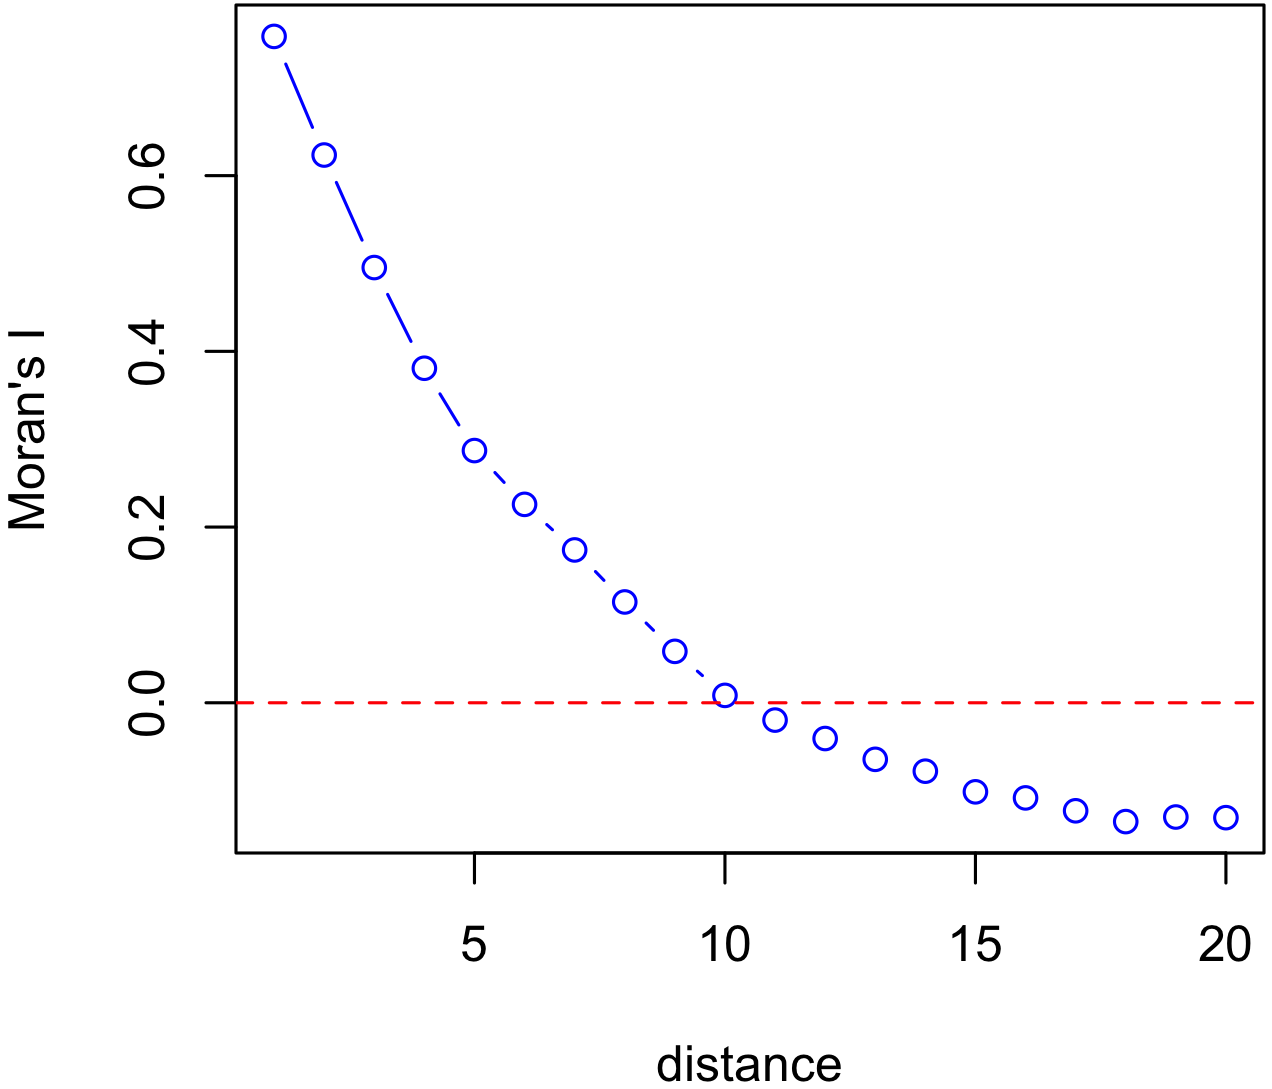
\includegraphics[width=0.6\textwidth]{images/spcorr.png}\\
  \pause
  \raggedright
  Insects with climate-associated traits exhibiting \alert{strong relationship with climate in their spatial autocorrelation} are likely to \alert{change distribution pattern} under climate change \footnotesize{(Dray et al. 2012)}
\end{frame}

\begin{frame}[fragile]
  \frametitle{Our research questions\protect\\ were two-fold}
  \begin{enumerate}
  \item which climate-associated traits and organism groups show the highest potential for changing distribution pattern?
  \medskip
  \pause
  \item which are most influential climatic aspects for traits and organism groups showing highest potential for changing distribution?
  \end{enumerate}
\end{frame}

\begin{frame}[fragile]
  \frametitle{We used biomonitoring data from 4,752 German stream sites \protect\\ and 35 global bioclimatic indices \small (Biss et al. 2006, Kriticos et al. 2012)}
  
  %Sections group slides of the same topic

  %\begin{minted}[fontsize=\small]{latex}
    %\section{Elements}
  %\end{minted}
  %for which the \emph{mtheme} provides a nice progress indicator \ldots
  %\begin{equation*}
    %C_{T,z} = \delta_{z,0} + \sum_{n=1}^{m=8}\delta_{z,n}S_{z,n} + e_z
    %\end{equation*}
    %\pause
  $\vcenter{\hbox{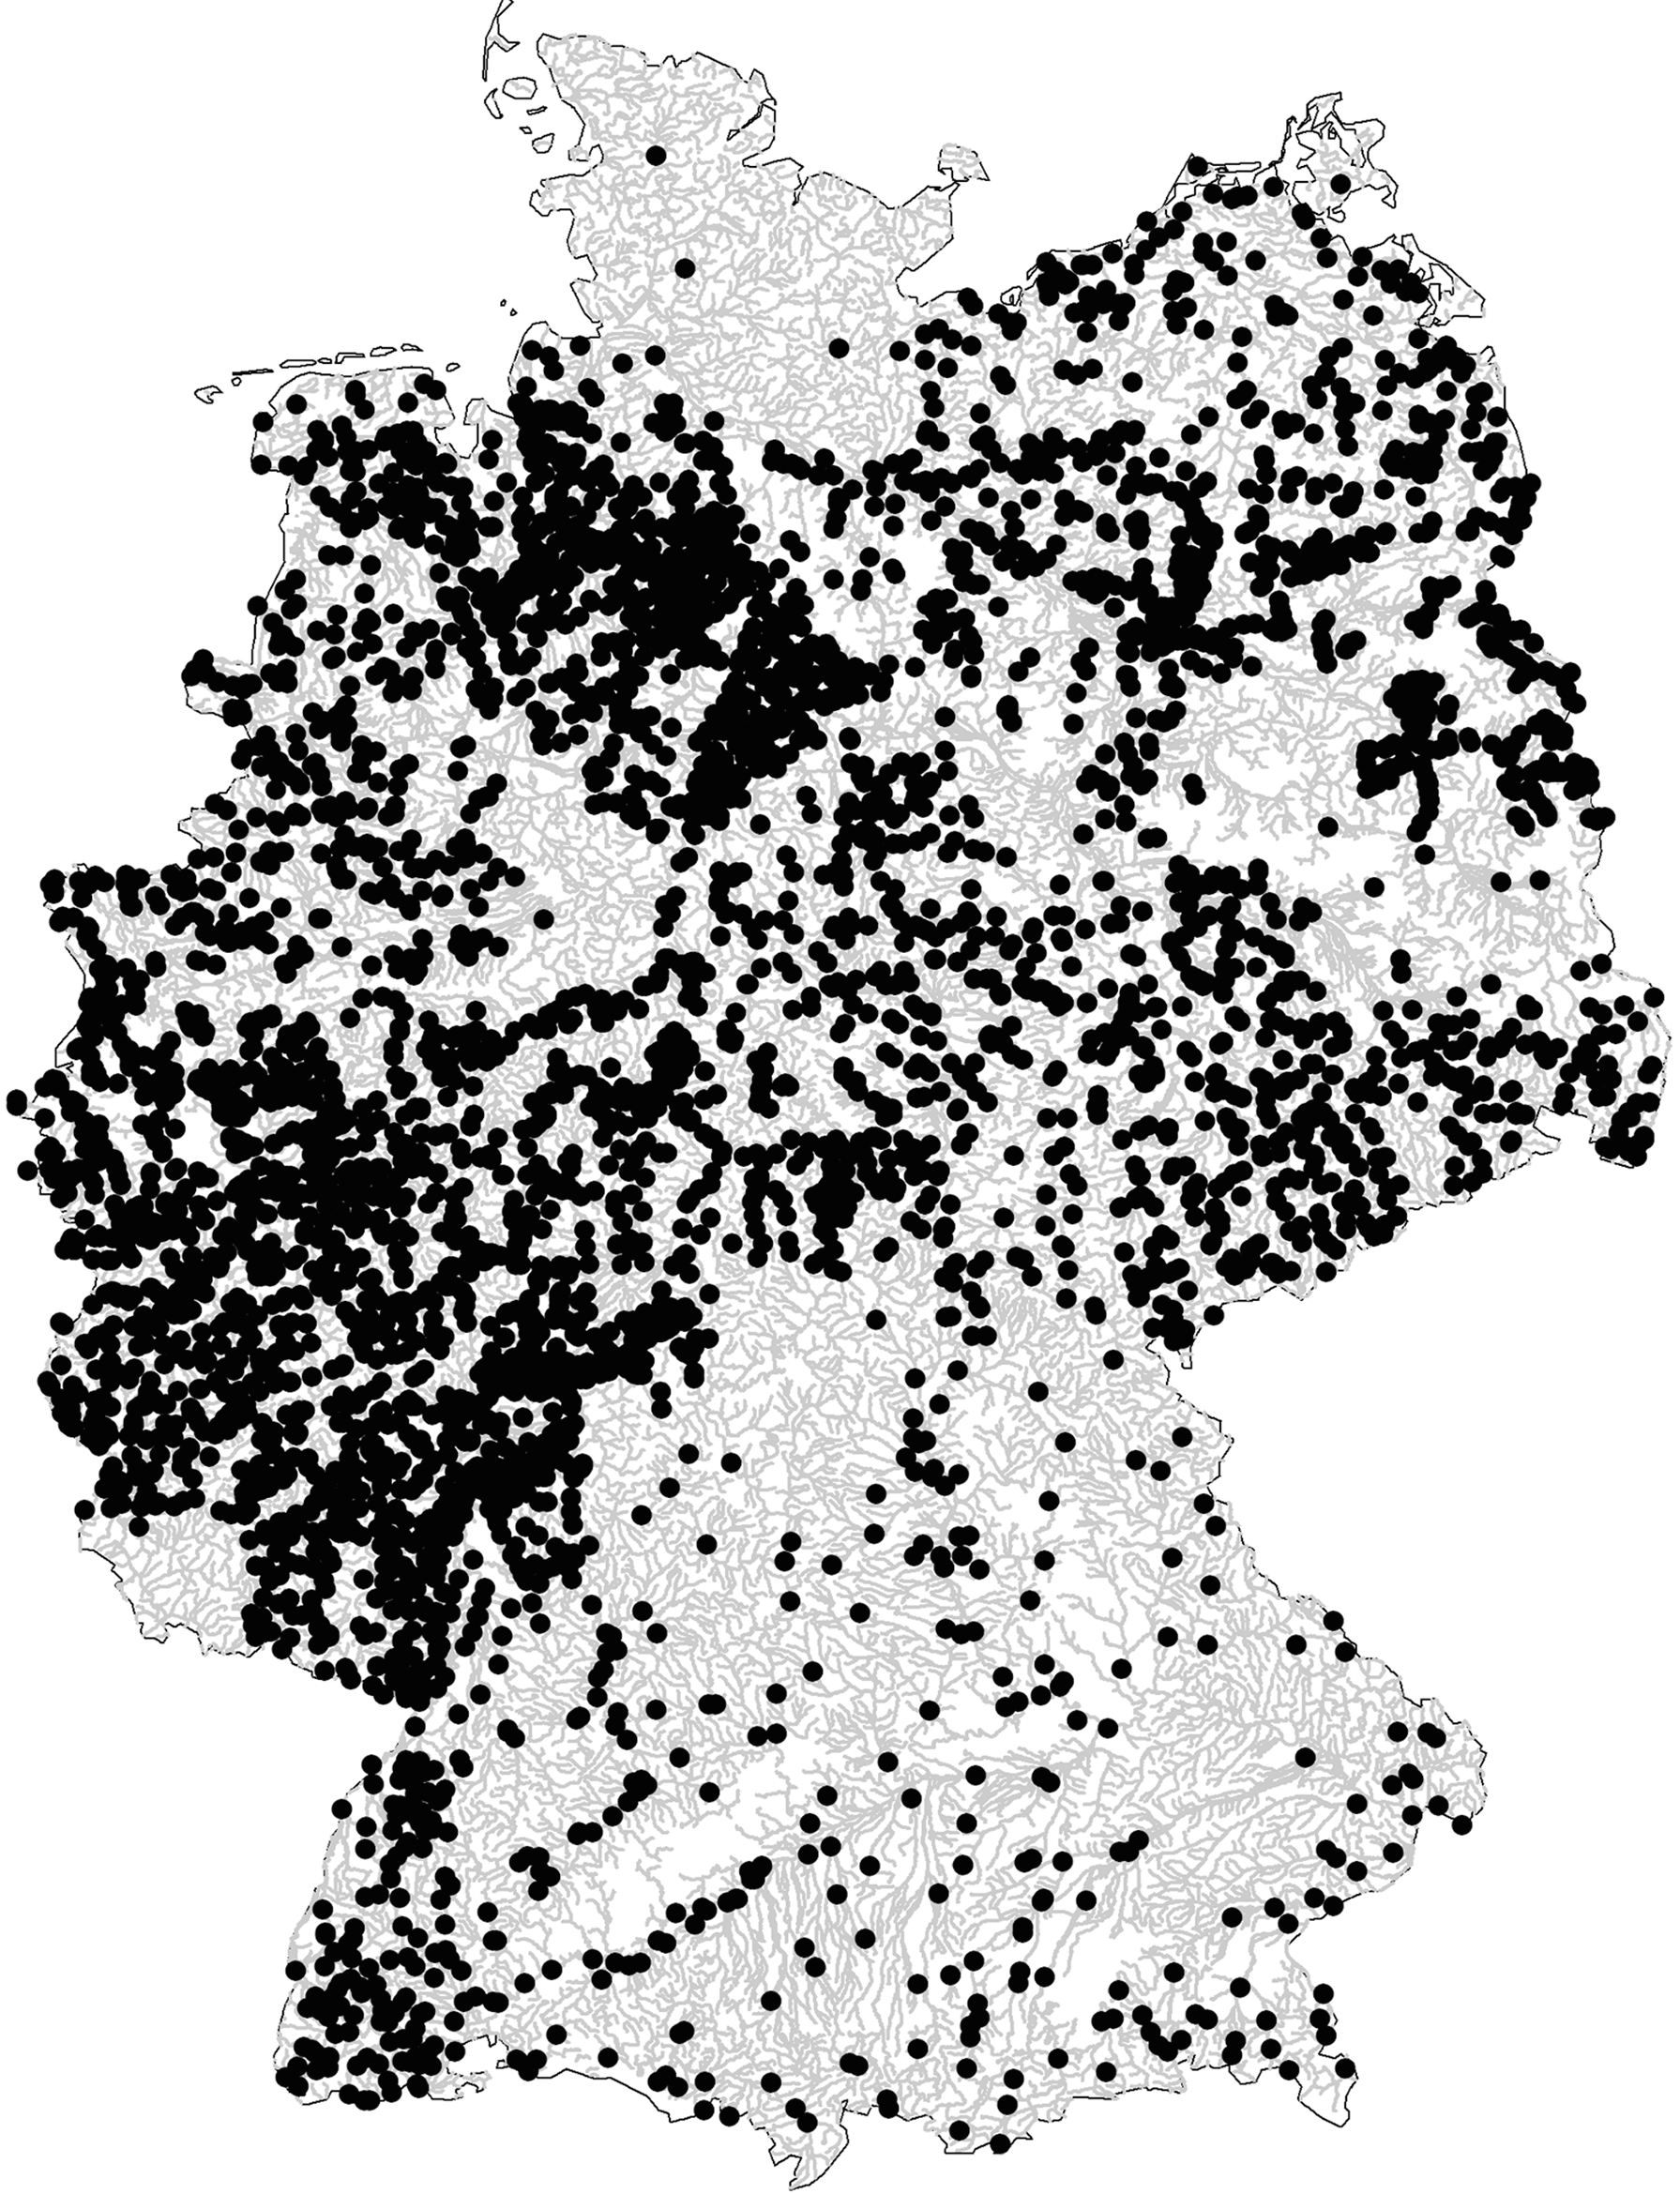
\includegraphics[width=0.48\textwidth]{images/Germany_Sites.png}}}$
  \hspace{5pt}
  $\vcenter{\hbox{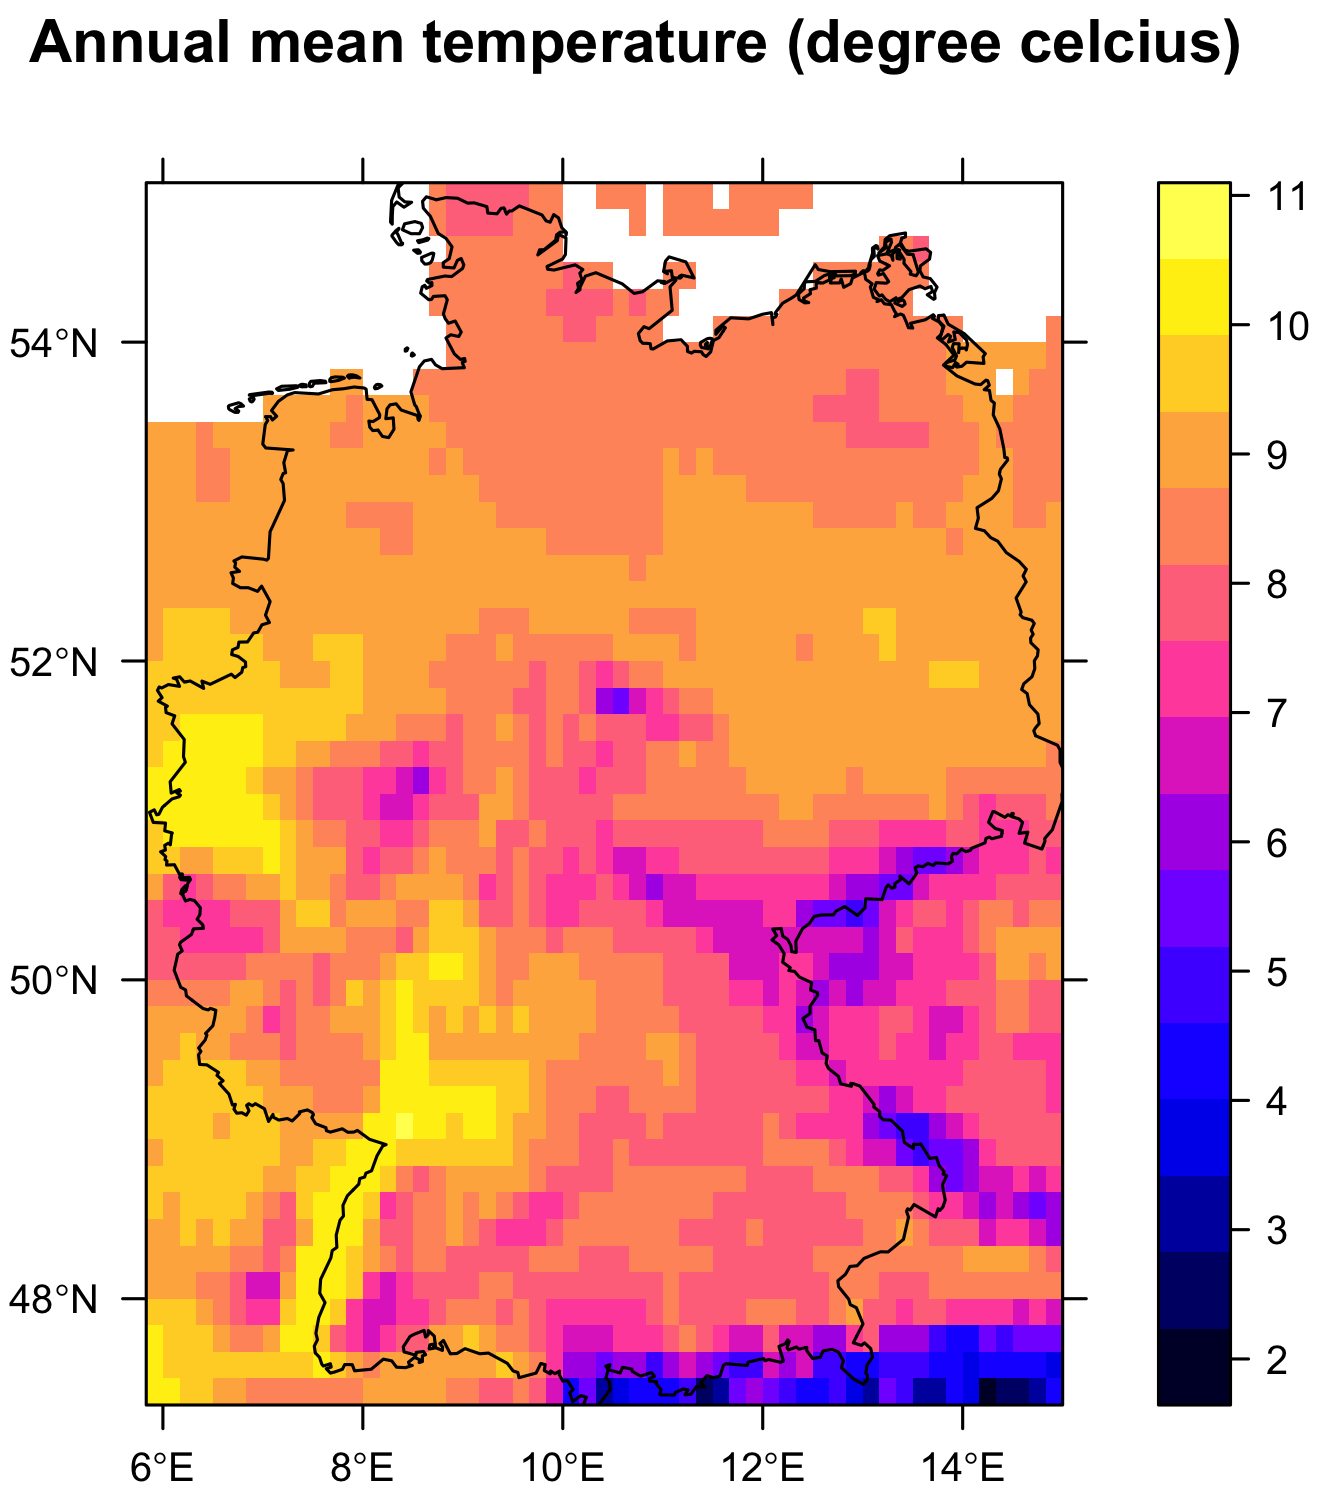
\includegraphics[width=0.48\textwidth]{images/Bioclim.png}}}$ \\
  \hspace{45pt} \alert{357,000 km\textsuperscript{2}} \hspace{110pt} \alert{18 km} 
  %\alert{Land cover \small{(ISCGM 2014)}} BL, AL, ML \hspace{6pt} \alert{Elevation \small{(Rodriguez et al. 2005)}} \\
  %\pause
  %\alert{Global soil properties \small{(Batjes 2000)}} SOC, SCC, WC, pH
\end{frame}

\begin{frame}[fragile]
  \frametitle{We selected climate-associated traits from 6 grouping features \protect\\ and 5 semi-aquatic orders}

  \centering
  $\vcenter{\hbox{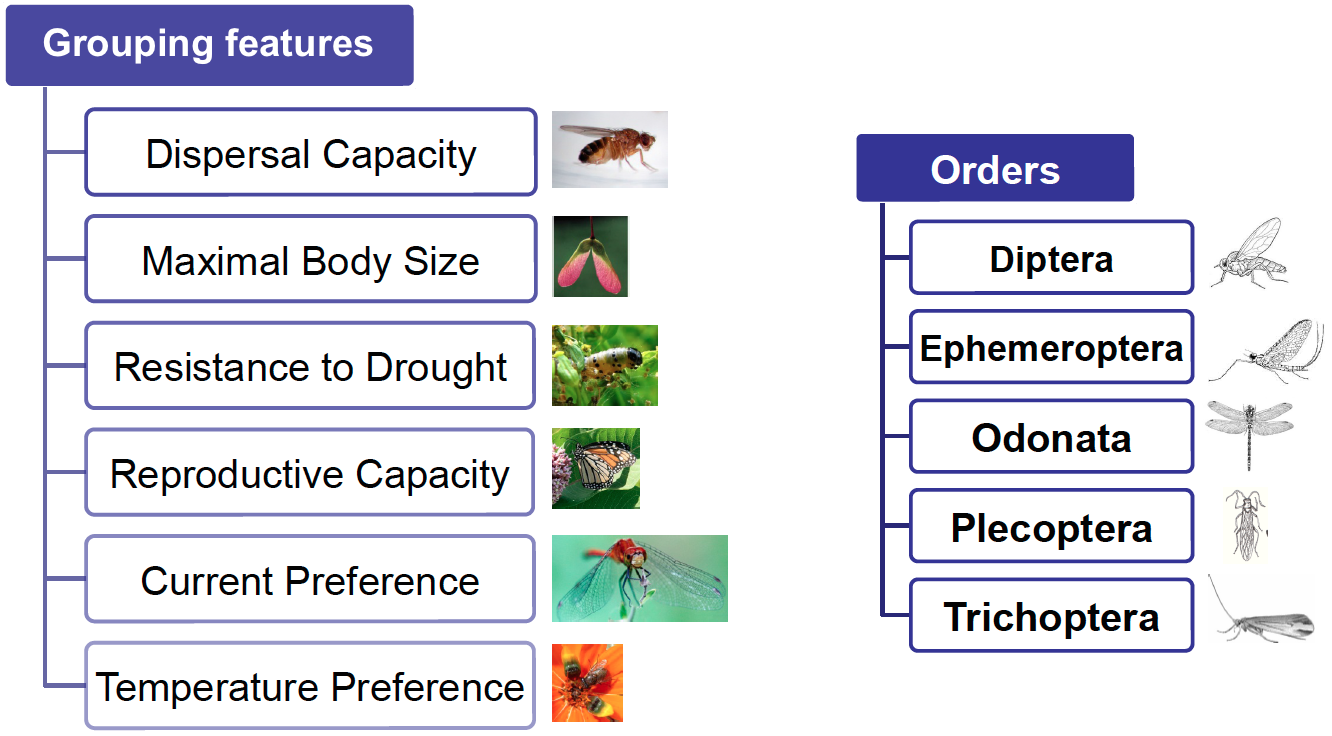
\includegraphics[width=1\textwidth]{images/Traits_Orders.png}}}$\\
    \vspace{10pt} Trait databases: \alert{freshwater ecology \footnotesize (Schmidt-Kloiber and Hering, 2015), \normalsize Tachet \footnotesize (Usseglio-Polatera et al. 2000)}\\
 
\end{frame}

\begin{frame}[fragile]
  \frametitle{We linked biomonitoring data with trait data\protect\\ and computed abundance-weighted traits \footnotesize (Schmera et al. 2014)}
  \pause
  \centering
  $\vcenter{\hbox{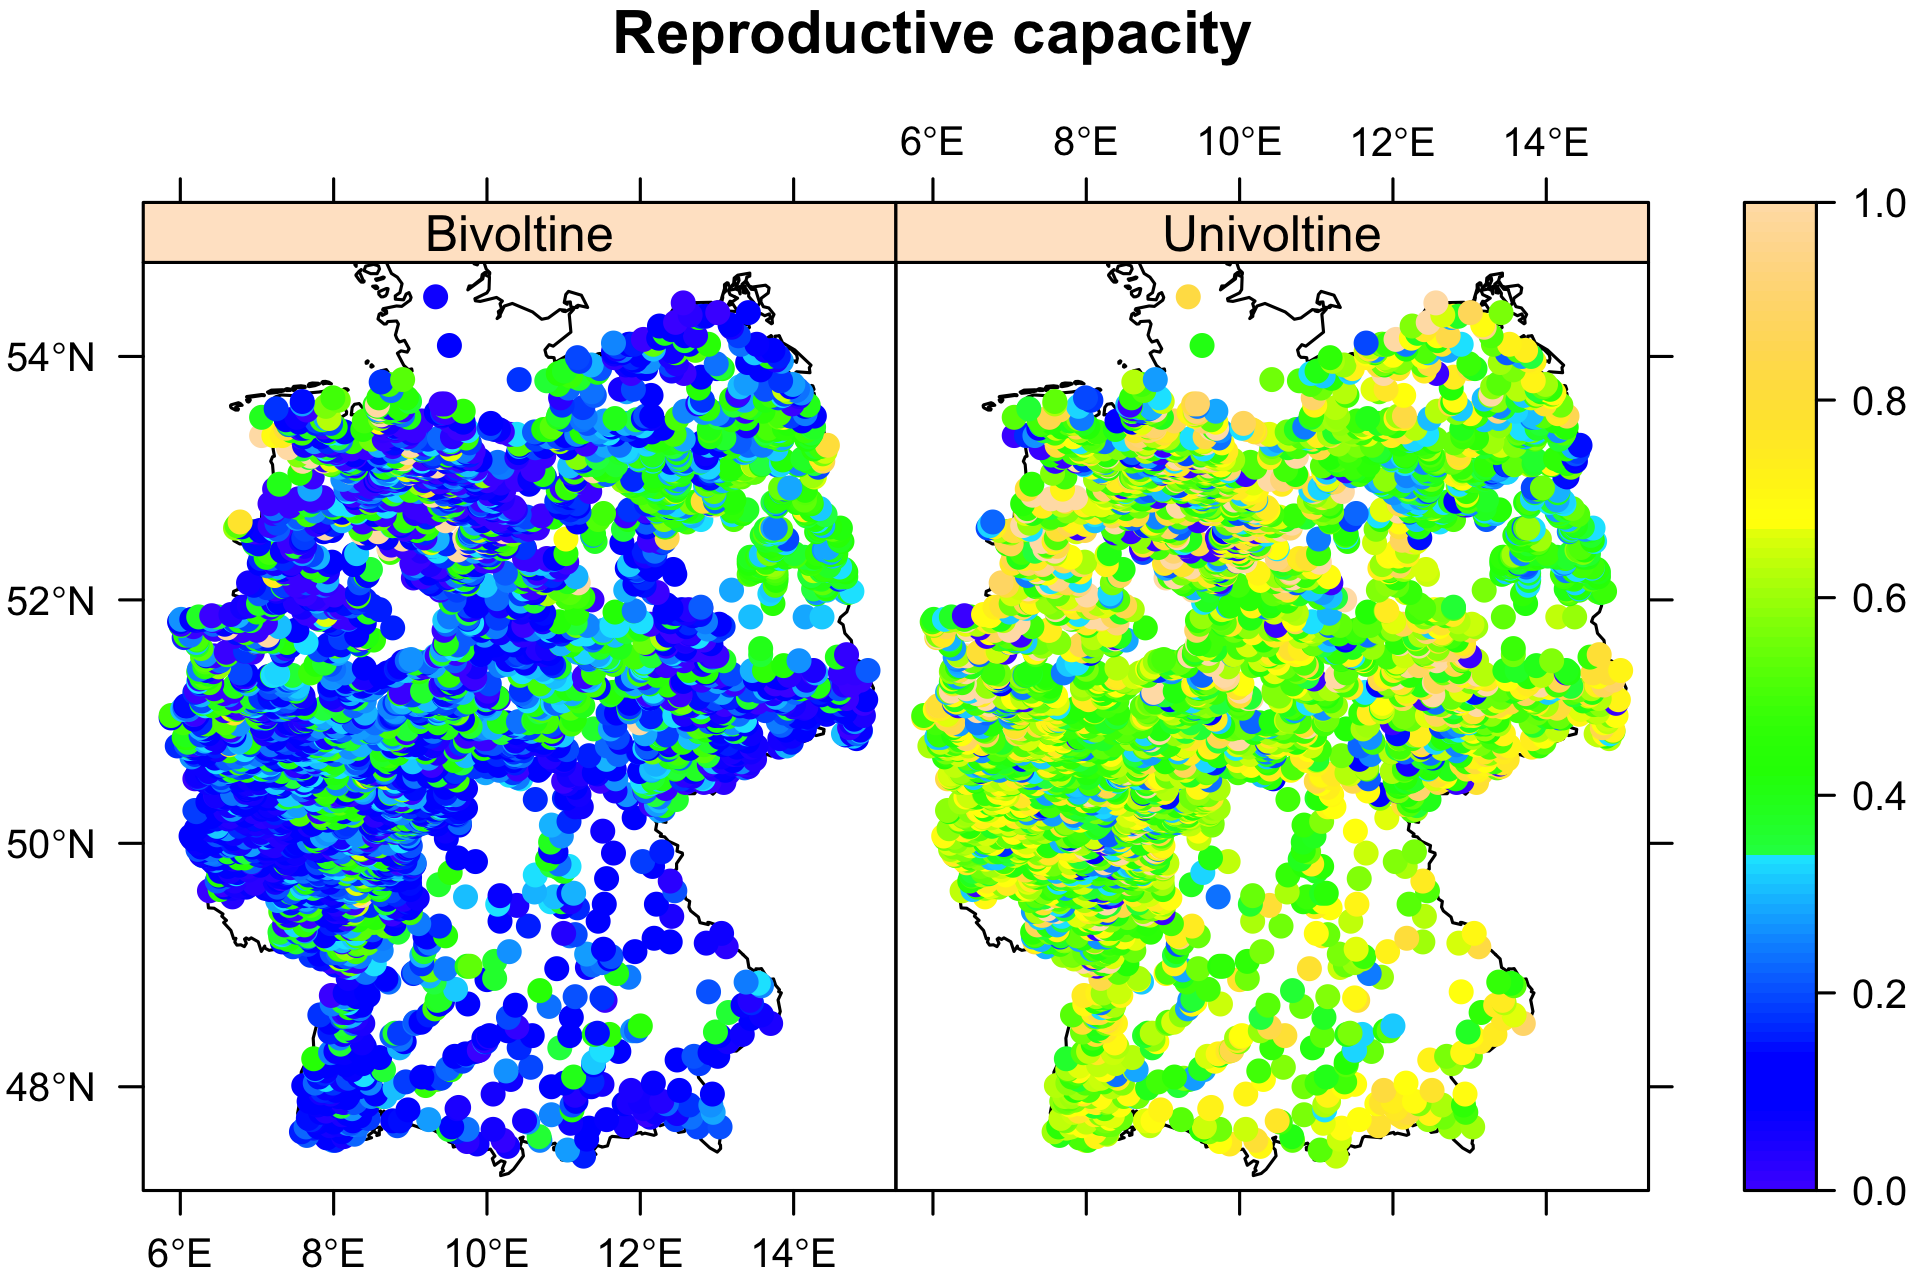
\includegraphics[width=1\textwidth]{images/Reprocapa.png}}}$
 
\end{frame}

\begin{frame}[fragile]
  \frametitle{We quantified the amount of spatial autocorrelation\protect\\ that is associated with bioclimatic indices \footnotesize (Schmera et al. 2014)}
  \begin{enumerate}
  \item Spatial autocorrelation \alert{(Global Moran's I)} in abundance-weighted traits
  \pause
  \item \alert{Trait-Climate model:} relationship between abundance-weighted traits and bioclimatic indices
  \pause
  \item Global Moran's I in the residuals of trait-climate model
  \pause
  \item Relationship between abundance-weighted traits and individual bioclimatic indices
  \end{enumerate} 
\end{frame}

\begin{frame}[fragile]
  \frametitle{59 \% spatial autocorrelation in abundance-weighted traits\protect\\was associated with bioclimatic indices}
  \pause
  Highest spatial autocorrelation was explained:
  \begin{itemize}
  \item in \alert{temperature preference (81 \%)} , particularly in insects with \alert{cold temperature preference (91 \%)} $\vcenter{\hbox{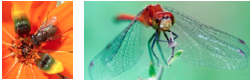
\includegraphics[width=0.15\textwidth]{images/Temperature.png}}}$
  \medskip
  \pause
  \item for \alert{Ephemeroptera (59 \%)}, particularly for \alert{Trichoptera with moderate temperature preference (97 \%)}  $\vcenter{\hbox{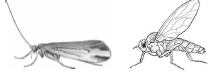
\includegraphics[width=0.15\textwidth]{images/Orders.png}}}$
  \medskip
  \pause
  \item Traits of \alert{temperature preference} showed strong covariation with underlying \alert{climate-associated traits} \\
  \pause
  e.g. \alert{low dispersal capacity, large body size (>4 cm), low reproductive capacity (semivoltine) and resistance to drought (egg diapause together explained 55 \% of cold temperature preference}
  \end{itemize}
\end{frame}

\begin{frame}[fragile]
  \frametitle{59 \% spatial autocorrelation in abundance-weighted traits\protect\\was associated with bioclimatic indices}
  \centering
  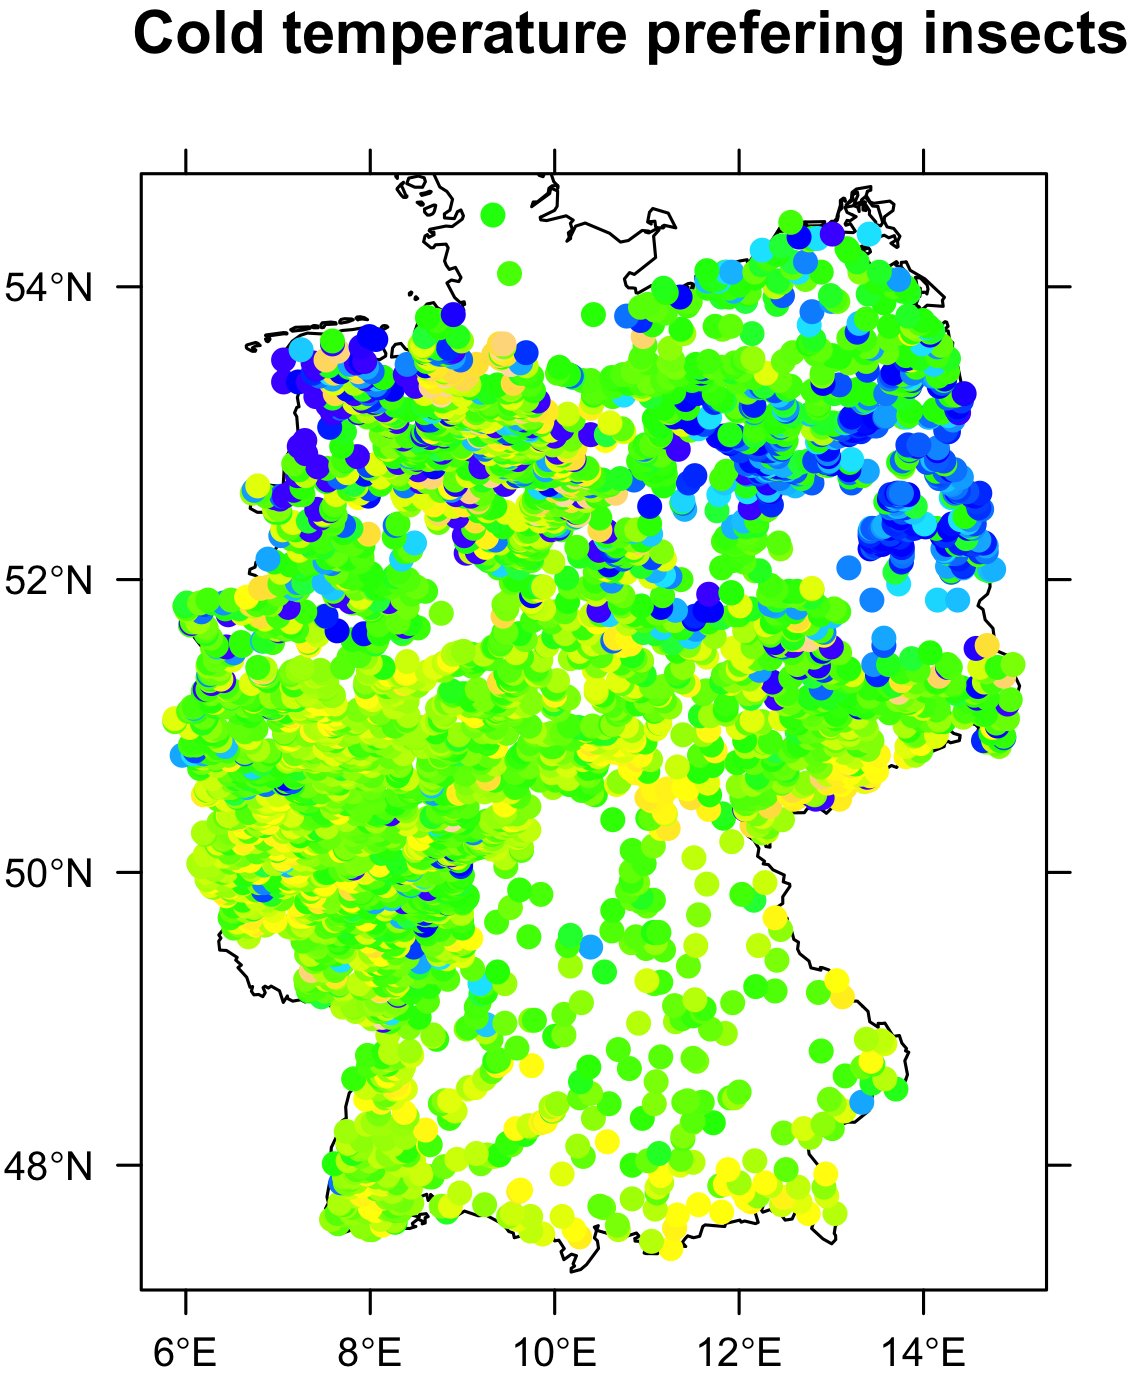
\includegraphics[width=0.45\textwidth]{images/Cold.png}
  \pause
  \hspace{2pt}
  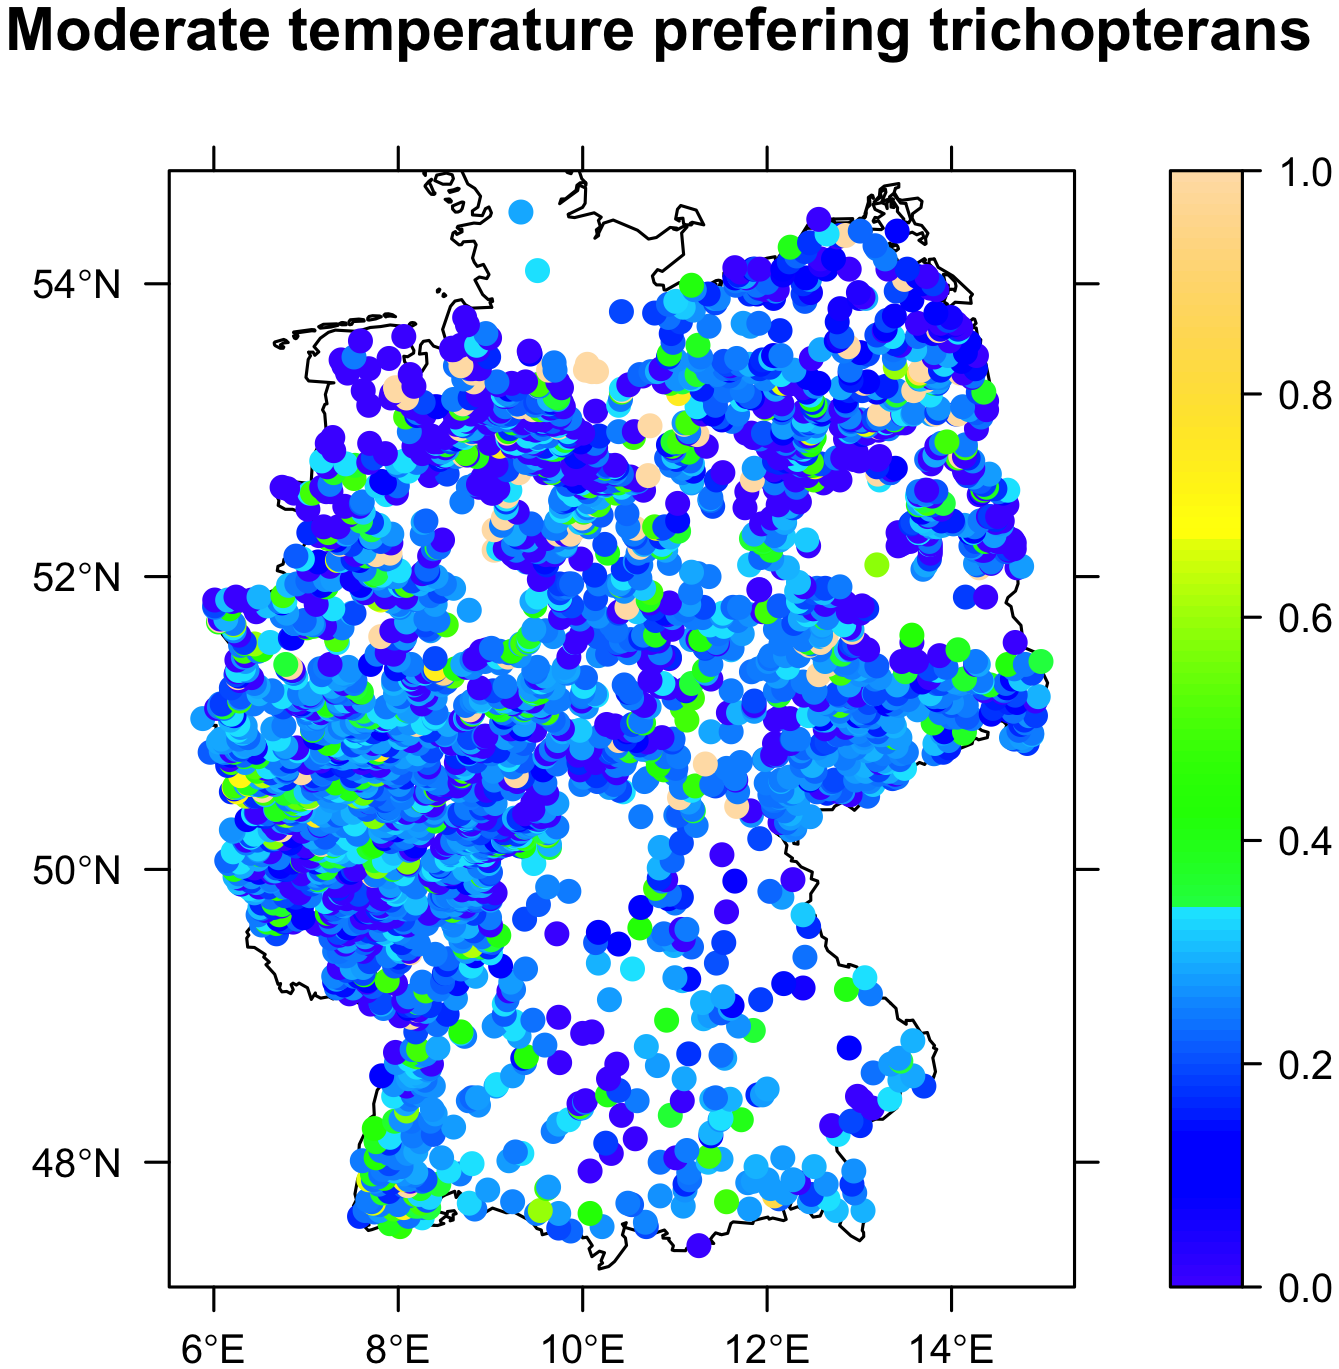
\includegraphics[width=0.535\textwidth]{images/Modetri.png}
  
\end{frame}

\begin{frame}[fragile]
\frametitle{Seasonal radiation and temperature\protect\\was the most influential bioclimatic aspect}
\begin{itemize}
\item \alert{Radiation seasonality (46 \%)} explained highest SA in cold temperature preferring insects
\pause
\item \alert{Radiation (65 \%) and mean temperature (64 \%) of the driest quarter} explained highest SA in moderate temperature preferring trichopterans
\end{itemize}
\pause
\centering
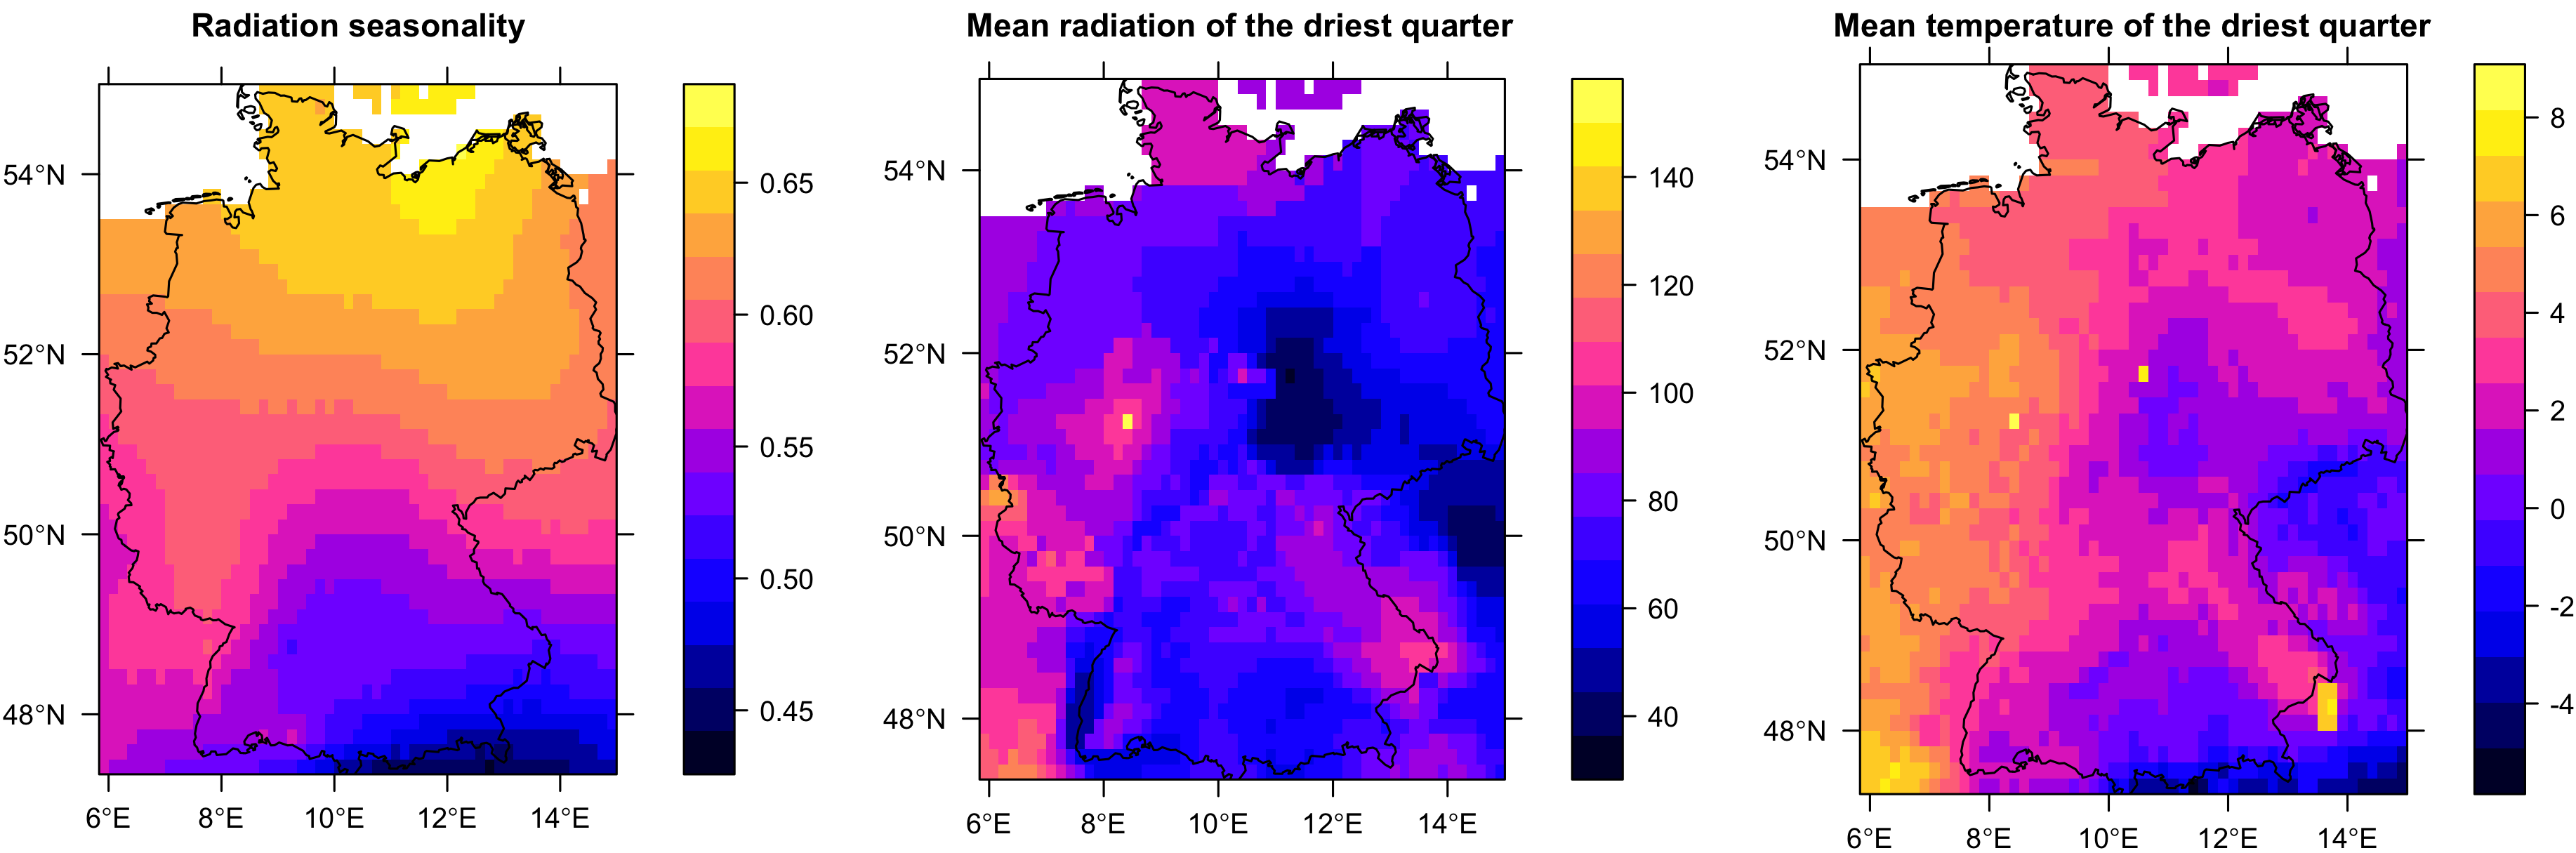
\includegraphics[width=1\textwidth]{images/Inf_Bio.png}
\end{frame}

\begin{frame}{We anticipate change in aquatic insect distribution pattern\protect\\ along the longitudinal gradient in Germany}
\begin{itemize}
\item \alert{Winter and summer temperature may increase in the South} \footnotesize{(Stocker et al. 2013)}
\pause
\item \normalsize \alert{Cold temperature preferring insects} mostly occur in the South\\
\pause
\vspace{10pt}
insects with low dispersal capacity \footnotesize{(Hershkovitz et al. 2015)}\\
\pause
\vspace{10pt}
\normalsize large-bodied insects \footnotesize{(Harrison et al. 2010, Verberk and Atkinson 2013)}\\
\pause
\vspace{10pt}
\normalsize \alert{hence, may shrink their distribution}
\pause
\medskip
\item \normalsize \alert{Moderate temperature preferring trichopterans} mostly occur in the North may extend their range \footnotesize{(Hering et al. 2009)}
\end{itemize}
\end{frame}

\begin{frame}{We anticipate change in aquatic insect distribution pattern\protect\\ along the longitudinal gradient in Germany}
\centering

\includegraphics[width=0.6\textwidth]{images/Brave.png}
\end{frame}

\plain{}{\small For more: Bhowmik and Schäfer 2015, PLOS ONE, 10(6): e0130025 \\
\vspace{30pt} \LARGE Thank you \\
\vspace{30pt} Questions?}

\end{document}
